

\chapter{MapReduce}
\label{MapReduce}

\section{Modell}

MapReduce ist ein generalisierter Ansatz für verteile Datenverarbeitung.
Zusätzlich wird mit MapReduce eine Laufzeitumgebung vorgeschlagen, welche für die automatische Verteilung und Parallelierung zuständig ist und außerdem Fehlerbehandlung, sowieso Kommunikation während der verteilten Berechnung abdeckt.
Folgende Übersicht basiert auf dem Paper \textit{MapReduce: Simplified Data Processing on Large Clusters} \cite{mapReduce}.


\begin{figure}[H]
	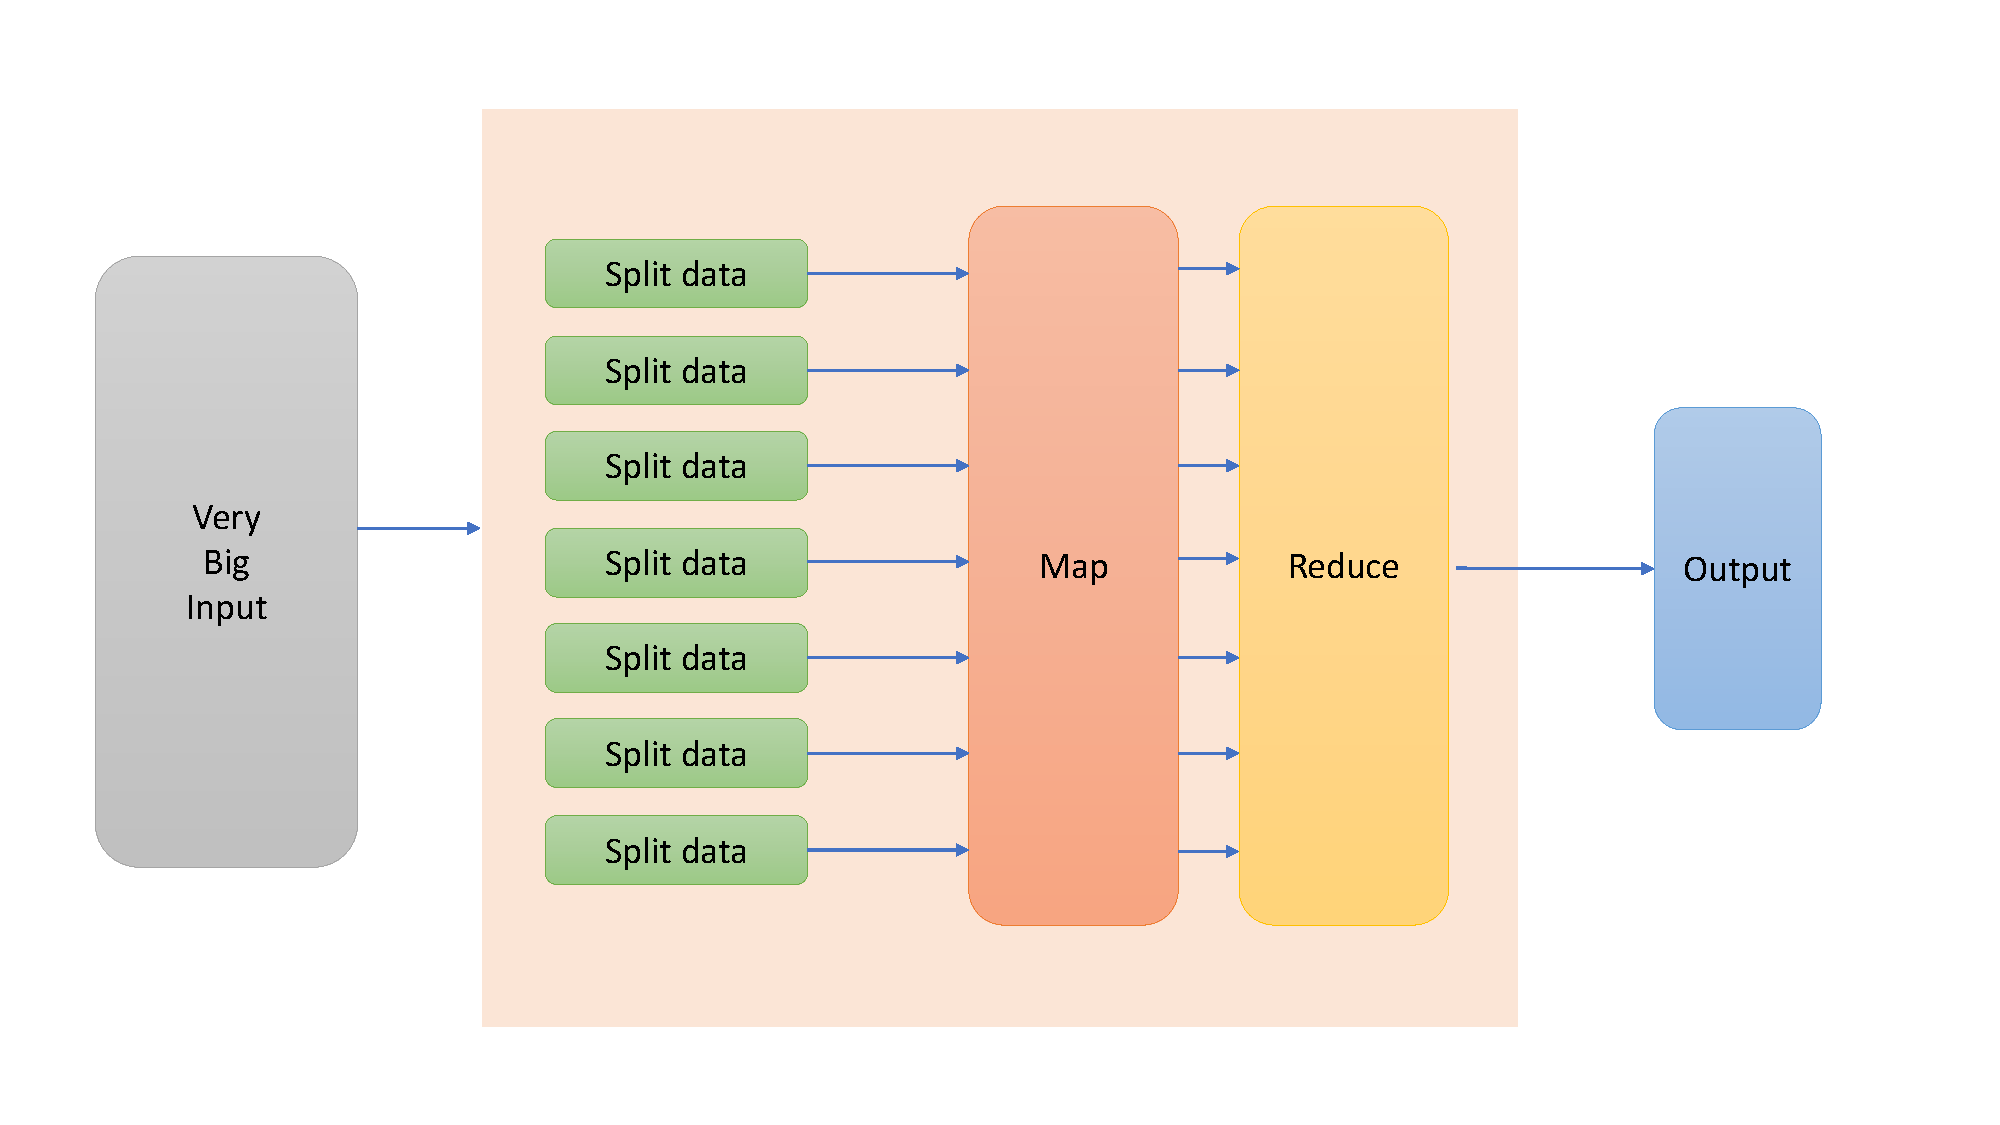
\includegraphics[width=\textwidth]{pics/mapReduce/overview}
	\caption{MapReduce Modell Übersicht}
\end{figure}


Um eine verteilte Berechnung und Verarbeitung zu vereinfachen, wird diese in zwei grobe Phasen aufgeteilt: Map und Reduce.
Für beide Phasen muss der Nutzer jeweils eine entsprechende Funktion definieren.
Der Input liegt als key/value Paare vor und MapReduce produziert wiederum key/value Paare als Ergebnis.
In der Map Phase werden aus den gegeben key/value Paaren Zwischenwerte berechnet, welche wiederum als key/value Paare vorliegen. Diese werden anschließend gruppiert und in der Reduce Phase weiterbehandelt.
In der Reduce Phase werden dann die berechneten Zwischenwerte für gleiche keys zusammengefasst und aggregiert.

Beispiel:
Für eine Vielzahl von vorliegenden Dokumenten soll die Wortanzahl ermittelt werden.
Dann könnten die Map und Reduce Funktionen wie folgt aussehen:

\begin{lstlisting}[language=json,firstnumber=1]
map(String key, String value):
	// key: document name
	// value: document contents
	for each word w in value:
		EmitIntermediate(w, "1");

reduce(String key, Iterator values):
	// key: a word
	// values: a list of counts
	int result = 0;
	for each v in values:
		result += ParseInt(v);
	Emit(AsString(result));

\end{lstlisting}

Die Map function gibt also einfach jedes Wort plus ein Anzahl, in diesem Falle einfach 1 zurück.
Anschließend würde die Reduce Funktion alle zurückgebenen Anzahlen für jedes Wort summieren.



\section{Implementation}

Für das MapReduce Interface sind laut Paper \cite{mapReduce} verschiedene Umsetzungen möglich, die sich an den  Ausführungsumgebungen ausrichten.
Im Paper wird dann eine Umsetzung für eine damals typisch eingesetzte Environment vorgestellt.
Als Ausführungsumgebungen werden große Cluster (Anzahl 100-1000 Knoten) von Computern mit durchschnittlicher Rechenleistung und Hauptspeicher genannt.
Folgend wird beschrieben wie die Verteilung der Map und Reduce Funktion in dieser Umgebung von Google implementiert wurde.
Auf den Knoten läuft ein verteiltes Dateisystem (GFS), welches ein Zugriff auf Dateien über das Netzwerk ermöglicht, ein Knoten jedoch dabei diese Dateien wie lokate Dateien behandeln kann.
Der Nutzer übermittelt den MapReduce-Job an ein Scheduling System, welches dann die Ausführung koordiniert.


\subsection*{Vorbereitungen}
Ein Knoten übernimmt die Aufgabe des Masters, welcher dann die weitere Ausführung und das Scheduling übernimmt.
Der übermittelte MapReduce-Job wird dann wie folgt in verschiedene Tasks aufgeteilt:
\begin{enumerate}
	\item
	Die Eingabedaten werden in M Parts gesplittet, pro Part wird später ein Map-Task ausgeführt.
	\item
	Die Reduce-Phase wird in R Reduce-Tasks aufgeteilt.
	Hierzu wird die Menge der möglichen Zwischenergebnisse
	durch eine Verteilungsfunktion in R Partitionen aufgeteilt.
\end{enumerate}
Diese Tasks werden den Workern dann dymamisch während der Ausführung zugeteilt.
Typische Zahlen sind: Z.B: M=200.000 R=4000, workers=2000

\subsection*{Ausführung der Map Phase}

In der Map Phase teilt der Master jedem freien Worker einen Map-Task zu.
Der Worker liest den zum Map-Task gehörenden Datenpart und führt darauf die Map-Funktion aus.
Hierbei werden (bis zu) R lokale Dateien (eine Datei pro Key) mit
Zwischenergebnissen lokal gespeichert.
Zum Schluss übermittelt der Worker den Speicherort der Zwischenergebnisse an den Master, damit diese später verteilt werden können.

\begin{figure}[H]
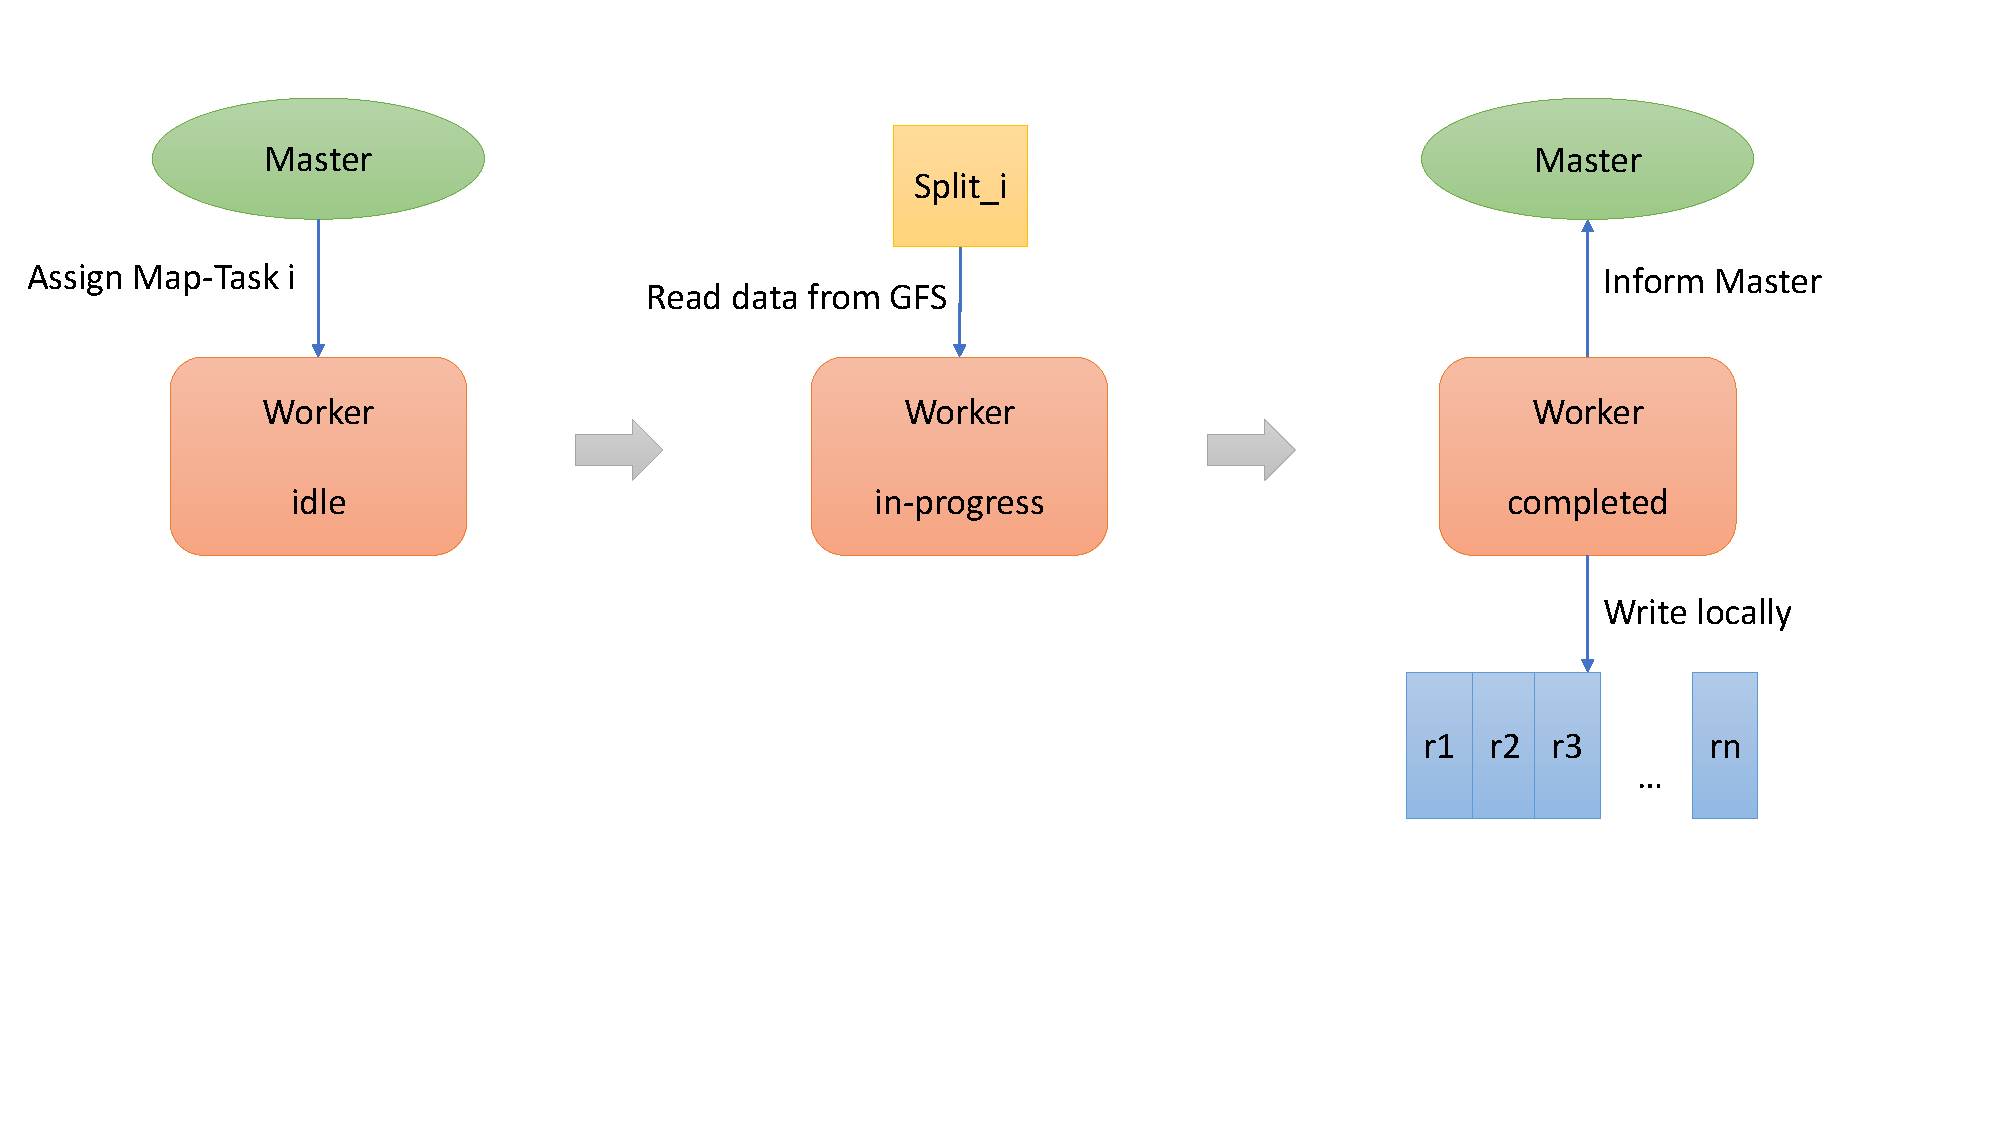
\includegraphics[width=\textwidth]{pics/mapReduce/mapassign}
	\caption{Ausführung eines Map tasks}
\end{figure}

\subsection*{Ausführung der Reduce Phase}

Der Master verteilt die Reduce-Tasks auf freie Worker und übermittelt dabei die Speicherorte der Zwischenergebnisse pro Key.
Dann liest der ausführende Worker die Zwischenergebnisse pro Key mittels RPC von den anderen Knoten, sortiert die Daten und wendet die vom User definierte Reduce-Funktion darauf an.
Anschließend wird ein Output-File mit dem Ergebnis ins verteilte Dateisystem geschrieben.


\begin{figure}[H]
	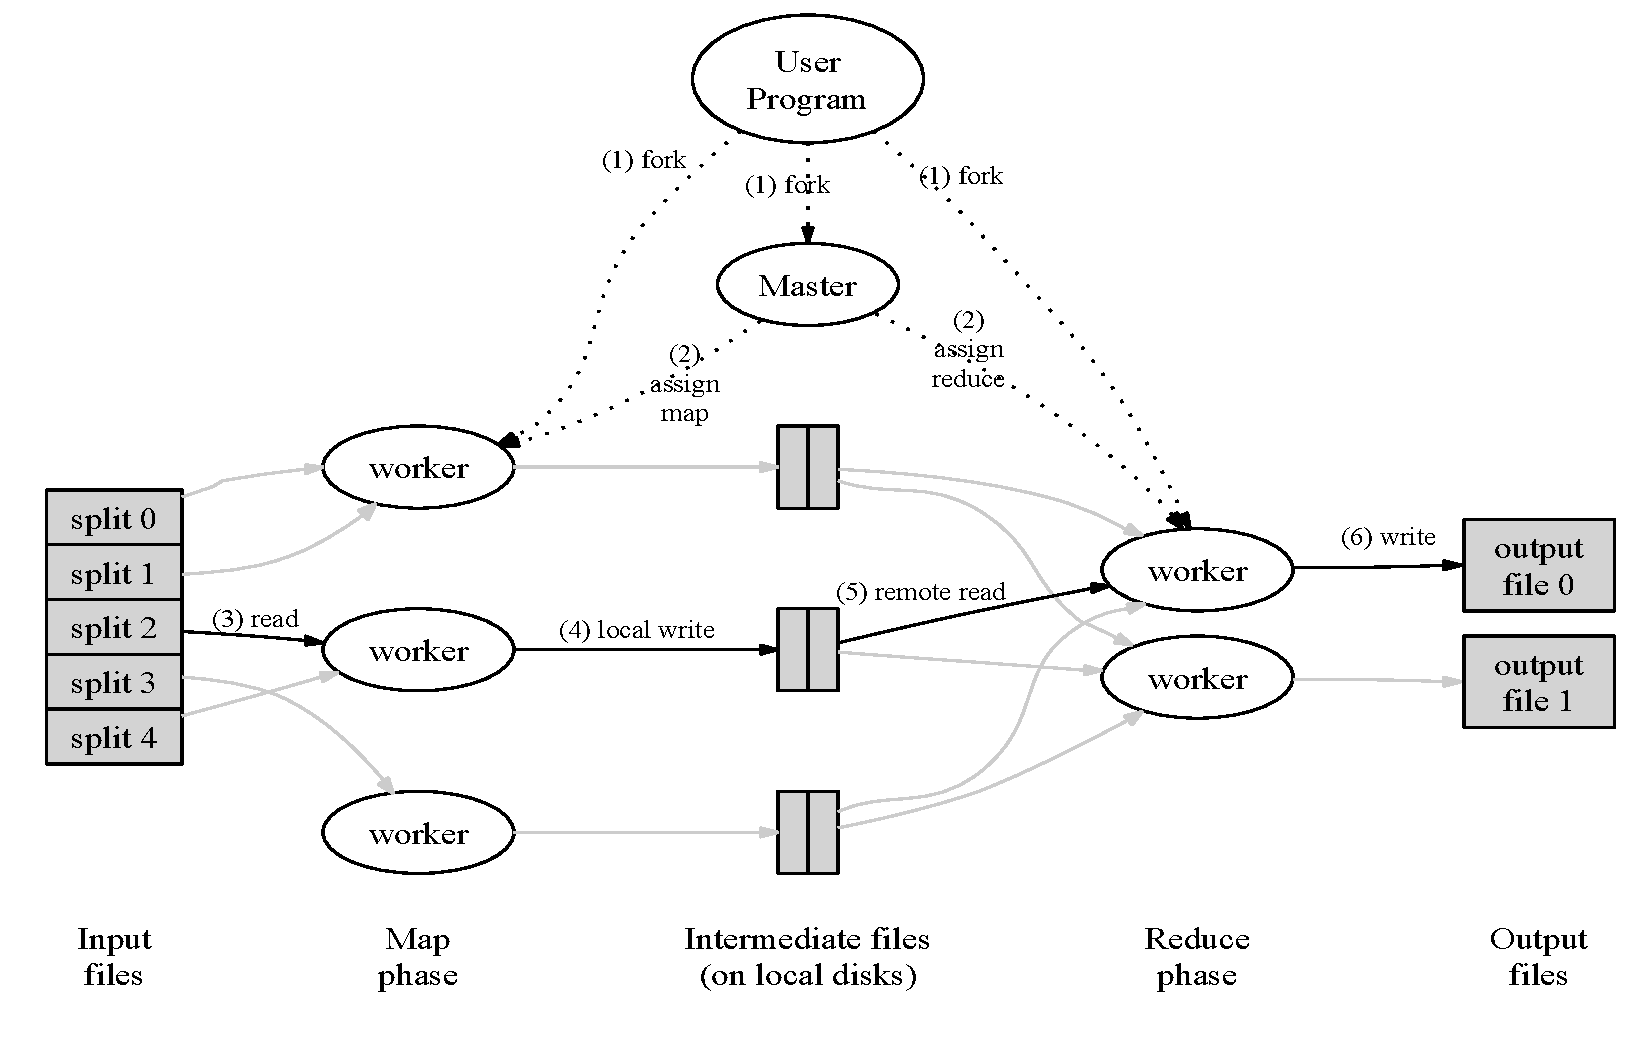
\includegraphics[width=\textwidth]{pics/mapReduce/mapreduce-osdi04e}
	\caption{Übersicht der gesament MapReduce Ausführungslogik}
\end{figure}


\subsection*{Fehlertoleranz}

Da MapReduce für den parallel Einsatzu auf vielen Knoten gedacht ist und einzelne Knoten ausfallen können, gibt es spezielle Fehlerfälle die betrachtet und behandelt werden.

Um ein Failure des Masterknotens aufzufangen, schreibt dieser periodisch Checkpoints vom derzeitigen Ausführungsstatus.
Tritt nun ein Fehler im Master auf, wird ein neuer Knoten als Master gestartet und die Ausführung vom letzten Checkpoint fortgeführt.

Jeder Workerknoten wird vom Master mittels Heartbeat periodisch auf Erreichbarkeit und Status abgefragt.
Wird ein ausgefallener Worker oder ein fehlerhafter Job erkannt, wird zwischen abgeschlossenen und nicht abgeschlossenen Job unterschieden.
Ein nicht abgeschlossener Map oder Reduce Task wird einfach auf einem anderen Worker neu gestartet.
Abgeschlossene Map Tasks werden auch erneut ausgeführt, da die Zwischenergebnisse lokal auf den Knoten liegen und diese entsprechend fehlen.
Abgeschlossene Reduce Tasks müssen nicht erneut ausgeführt werden, weil die Ergebnisse im verteilten Dateisystem gespeichert werden.


\section{Refinements}

Zur eigentlichen Ausführungslogik gibt es noch weitere Refinements, die die Ausführung optimieren.
\subsection*{Combiner}
In der Map Phase entstehen oftmals Wiederholungen von Zwischenergebnissen.
Im Wordcount Beispiel:
\begin{verbatim}
(foo bar bar bar) → (foo, 1) (bar, 1) (bar, 1) (bar, 1)
\end{verbatim}

Ein Worker kann nach Abschluss einen Map-Tasks die Zwischenergebnissen pro key mittels Combine Funktion zusammenfassen.
Z.B.
\begin{verbatim}
(foo, 1) (bar, 1) (bar, 1) (bar, 1) → (foo, 1) (bar, 3)
\end{verbatim}


\subsection*{Partitioning Function}

Die Nummer der Reduce-Tasks wird von Nutzer festgelegt.
Nun gibt es eine default Partitioning Function (hash(key) mod R),
welche die Zwischenergebnisse nach Keys den Reduce-Tasks zuordnet.
Durch die default PF werden meist gut verteilte Partitionen generiert,
allerdings kann der Nutzer auch eigene Verteilungsfunktionen definieren.

\subsection*{Datenlokalität}

Die Inputdaten werden im verteilten Dateisystem in Blöcke geteilt und repliziert auf verschiedenen Knoten gespeichert.
Da diese Blöcke später den MAP-Tasks zugeordnet sind, versucht der Master die Tasks so zu verteilen, dass die benötigten Blöcke auf den zugeordneten Knoten oder zumindest physisch in der Nähe liegen.
Hierdurch wird der Netzwerkdurchsatz während der Taskausführung reduziert und eine Ausbremsung verhindert.


\subsection*{Backup Tasks}

Einzelne, aufgrund Nebeneffekten sehr langsame Knoten, können den Gesamtprozess aufhalten, besonders wenn diese zum Ende eine Phase auftreten.
Um dies zu vermeiden, werden zum Ende einer MapReduce Phase Tasks welche noch nicht abgeschlossen sind, repliziert und auf mehren Knoten parallel ausgeführt.
Der erste abgeschlossene Task 'gewinnt' und langsame Knoten werden übergangen.


\section{Probleme und Nachteile von MapReduce}

MapReduce und Spark (siehe nächstes Kapitel) ermöglichen die parallele und verteile Verarbeitung von riesigen Datenmengen.
Allerdings speichert und verarbeitet MapReduce alle Daten auf der Platte, während Spark durch eine in-memory Verarbeitung bis zu 100 mal schneller ist.
Auch bei iterativer Verarbeitung kann Spark durch die RDDs mehrere Operationen im Speicher ausführen, 
während MapReduce für jede Iterationen einen gesamten Durchlauf anstößt.
MapReduce zwingt den Nutzer die Verabeitung der Daten in eine Map- und eine Reduce-Funktion aufzuteilen, Spark bietet dem Nutzer hier viel mehr Komfort, weil zusätzliche Operationen möglich sind und eine High Level API anbietet. 

Zusätzlich bietet Spark eine Möglichkeit Streams zu verabeiten, was gerade in Hinsicht auf unseren Anwendungsfall, nämlich die Verarbeitung und live Analyse von Twitterdaten interessant ist. 

